\section{Groups acting on $\mathbb{R}$-Trees}
\todo[color=green!40]{Hello Lorna, Talia here! I fixed a few tiny typos and punctuation things. For anything bigger, I will add comments in boxes. Take a look when you have a chance, and feel totally free to ignore any of my suggestions!}

In this section we will discuss a class metric spaces called $\mathbb{R}$-trees, which admit interesting group actions. These actions arise in proofs across the field of geometric group theory, in areas from hyperbolic groups to \textcolor{red}{something else??}. We will give an introduction to these spaces and the groups which act on them, followed by an overview of some of their applications. We also aim to highlight different ways in which Bass-Serre theory fails for $\mathbb{R}$-trees. Much of this section follows \cite{Bestvina_trees}.
\subsection{Definition and Basic Examples}
\begin{definition}
    A metric space $(X,d)$ is an \emph{$\mathbb{R}$-tree} if for every pair of points $x,y\in X$ there is a unique geodesic from $x$ to $y$.
\end{definition}

The following follows immediately from the definition, and is sometimes used as an alternative characterisation:

\begin{proposition}
    A metric space is an $\mathbb{R}$-tree if and only if it is 0-hyperbolic.
\end{proposition}

We now give some simple examples of $\mathbb{R}$-trees.

\begin{example}
    Any tree $T$ with the metric defined by identifying each edge with the interval $[0,1]$ is an $\mathbb{R}$-tree.
\end{example}

\begin{example}\label{Paris}
    $\mathbb{R}^2$ with the \textit{Paris metric} is an $\mathbb{R}$-tree. This is the metric $d$ defined by\[d(x,y)=d_E(x,y)\]if $x$ and $y$ lie on the same line through the origin, and\[d(x,y)=d_E(x,0)+d_E(0,y)\] otherwise (here $d_E$ is the Euclidean metric on $\mathbb{R}^2$). It can be thought of as train lines in France which all go through Paris.
\end{example}

\begin{example}\label{xtrains}
    We can define a similar metric on $\mathbb{R}^2$ to that given in Example \ref{Paris} above by treating the $x$-axis and every vertical line as our train lines. Now the geodesic between two points must go \todo[color=green!40]{Changed this to a non-breaking space using \(\sim\) in LaTeX. Nice examples!}\textit{via.}~the $x$-axis. Note that there is no underlying simplicial graph for this $\mathbb{R}$-tree, so in particular we have shown that $\mathbb{R}$-trees are slightly more general than simplicial trees with metrics.
\end{example}

\subsection{Group Actions}
Bass-Serre Theory gives a convenient way to study groups acting on simplicial trees; in particular Theorem \ref{structuretheorem} says that a group $G$ acting on a tree $X$ can be viewed as the fundamental group of $G\backslash X$. However, this fails in general for $\mathbb{R}$-trees. For example, let $X$ be the $\mathbb{R}$-tree described in Example \ref{xtrains}, and let $G$ be the trivial group acting on $X$. Then the quotient $G\backslash X$ is $X$, which is not a simplicial tree. \cite{Levit_rtrees} gives construction which aims to generalise to $\mathbb{R}$-trees. Here we instead study group actions on $\mathbb{R}$-trees using other methods.

Isometries of $\mathbb{R}$-trees have a classification analogous to that of isometries of hyperbolic space. 
\begin{definition}
    Let $G$ be a group acting by isometries on an $\mathbb{R}$-tree $T$. The \emph{translation length} of $g\in G$ is \[\lVert g\rVert=\underset{x\in T}{\text{inf}}d(x,g(x)).\]
    \begin{itemize}
        \item If $\lVert g\rVert=0$, $g$ is \emph{elliptic},
        \item If $\lVert g\rVert>0$, $g$ is \emph{hyperbolic}.
    \end{itemize}
\end{definition}

It is often useful to classify these isometries in terms of their invariant sets.
\begin{definition}
    Let $g$ be an isometry of an $\mathbb{R}$-tree $T$. Its \emph{characteristic set} is \[C_g = \{x\in T:d(x,g(x))=\lVert g \rVert\}.\]
\end{definition}
The proof of the following follows the same argument as the proof outline given in \cite{CullerMorgan}.
\begin{proposition}
    Let $g$ be an isometry of an $\mathbb{R}$-tree $T$. Then $C_g$ is invariant under the action of $g$ and is a closed, non-empty subtree of $T$. Also,
    \begin{itemize}
        \item if $g$ is elliptic, $C_g$ is fixed by $g$,
        \item if $g$ is hyperbolic, $C_g$ is isometric to $\mathbb{R}$, and is called the \emph{axis} of $g$. $g$ acts on its axis by translation by $\lVert g\rVert$.
    \end{itemize}
\end{proposition}
\begin{proof}
    In the elliptic case, $g$ clearly fixes $C_g$. We will show later that in this case $G_g$ is non-empty, (i.e. $g$ has a fixed point). Since $g$ is an isometry, if it fixes two points $x$ and $y\in T$, it must also fix the unique geodesic between them, so $C_g$ is connected. Similarly, if it fixes every point on a geodesic it must also fix the endpoints. Hence $C_g$ is a closed subtree as required.

    Now suppose $g$ is hyperbolic. In particular it has no fixed points. Consider a point $x\in T$. There is a unique arc $\alpha$ from $x$ to $g(x)$, with subarcs $\alpha \cap g(\alpha)$ and $\alpha \cap g^{-1}(\alpha)$. Let $m$ be the midpoint of $\alpha$ and suppose that $m\in \alpha \cap g(\alpha)$. Then $g(m)$ is a point in $\alpha$ which is $\frac{\ell(\alpha)}{2}$ away from $g(x)$, so we have $g(m)=m$, a contradiction to the hyperbolicity of $g$. A similar argument gives $m\notin \alpha \cap g^{-1}(\alpha)$. Denote by $\beta$, the subarc of $\alpha$ connecting $g(\alpha)$ to $g^{-1}(\alpha)$. Since in particular $m\in \beta$, we know that $\beta$ has positive length. If a point $p$ has $p\in \beta \cap g(\beta)$, $p$ must be an endpoint of $\beta$, since \[\beta\cap g(\beta)\subseteq\alpha\cap g(\alpha)\subseteq g(\alpha)\] and $\beta\cap g(\alpha)$ is a single point. Similarly the only point where $\beta$ meets $g^{-1}(\beta)$ is at its other endpoint. Repeating this argument inductively shows that \[C=\underset{n\in\mathbb{Z}}{\bigcup}g^n(\beta)\] is an arc in $T$ which is isometric to $\mathbb{R}$. In particular this is a closed subtree, and $g$ acts on it by translation by $\ell(\beta)$, so it is also invariant under the action of $g$. To show that $C=C_g$, note that for any point $y\in T$, $y$ has a closest point in $C$, denoted $c$. We have $d(y,c)=d(g(y),g(c))$ (so $g$ is `moved along' \todo[color=green!40]{Fixed the apostrophe (both were right-handed).} $C$ by the same amount as $c$), which implies that \[d(y,g(y))=d(y,c)+\ell(\beta)+d(g(c),g(y))=\ell(\beta)+2d(y,C).\] This means that $C=C_g$ and $\lVert g\rVert=\ell(\beta)$.

    Finally, since we have shown that if $g$ has no fixed points in $T$, then $\lVert g\rVert>0$, we can say that an elliptic element necessarily has a fixed point, and so $C_g$ is also non-empty in that case.
\end{proof}

We will mostly be concerned with \textit{non-trivial} group actions:
\begin{definition}
    The action of a group $G$ on an $\mathbb{R}$-tree by isometries is \emph{non-trivial} if no point in $T$ is fixed by every element of $G$.
\end{definition}

Also of interest are \textit{stable} actions:
\begin{definition}
    The action of a group $G$ on an $\mathbb{R}$-tree by isometries is \emph{minimal} if it has no proper $G$-invariant subtree.
\end{definition}

\begin{definition}
    Let $G$ be a group acting by isometries on an $\mathbb{R}$-tree $T$. A  non-degenerate subtree $S$ of $T$ (i.e. a subtree which is non-empty and not a single point) is \emph{stable} if for every subtree $S'\subset S$, \[\text{Fix}(S')=\text{Fix}(S)\] where Fix($S$) denotes the pointwise stabiliser of $S$. The action of $G$ is \emph{stable} if it is non-trivial, minimal, and every non-degenerate tree $T$ has a stable subtree.
\end{definition}

An important example of when $\mathbb{R}$-trees arise is as limits of hyperbolic metric spaces. To find a limit of spaces, we first need to define an underlying metric. This subsection is covered in more detail in \cite{BridsonSwarup}

\begin{definition}
    An $\epsilon$\emph{-approximation} between two metric spaces $X$ and $Y$ is a set $R\subseteq X\times Y$ such that:
    \begin{itemize}
        \item Every point in $X$ any $Y$ appears in some element of $R$, and
        \item If $(x,y),(x',y')\in R$ then \[\lvert d_X(x,x')-d_Y(y,y')\rvert<\epsilon.\]
    \end{itemize}
    If there exists an $\epsilon$-approximation between $X$ and $Y$, write $X\sim_\epsilon Y$. The \emph{Hausdorff-Gromov distance} between $X$ and $Y$ is \[D_H(X,Y)=\inf\{\epsilon:X\sim_\epsilon Y\}\] (and is infinite if no such $\epsilon$ exists).
\end{definition}

\begin{theorem}\label{limittrees}
    Let $X_i$ be a sequence of compact metric spaces such that $X_i\rightarrow X$ in the Hausdorff--Gromov\todo[color=green!40]{Changed the hyphen to an en-dash using --.} metric.
    \begin{enumerate}
        \item If every $X_i$ is a geodesic metric space then so is $X$,
        \item If $X_i$ is $\delta_i$-hyperbolic for each $i$, and $\delta_i\rightarrow 0$, then $X$ is an $\mathbb{R}$-tree. 
    \end{enumerate}
\end{theorem}

The proof (in \cite{Bestvina2}) is by simple hyperbolic geometry.
%probably not worth proving here :(
% \begin{proof}
%     See \cite{} for the proof of (1).

%     To prove (2), we first want to show that for every $x,y\in X$ there is a unique geodesic from $x$ to $y$. By (1) we know that there is at least one geodesic; denote this $[x,y]$, and suppose there is also some other geodesic. Let $z$ be the midpoint of this second geodesic, so we have a triangle with vertices $x,y$ and $z$. In the $X_i$ we have triangles which converge to this triangle, say with vertices $x_i,y_i$ and $z_i$. In this triangle in $X_i$, let $y_i'$ and $x_i'$ be the points on the edges $[x_i,z_i]$ and $[z_i,y_i]$ respectively which are at equal distance from $z_i$, and such that the remaining length of these edges sums to $d(x_i,y_i)$. Let $z_i'$ be the point on $[x_i,y_i]$ which divides it into this sum (see Figure \textcolor{red}{picture}). Then we have $d(x_i,z_i')=d(x_i,y_i')$, $d(y_i,z_i')=d(y_i,x_i')$, and $d(z_i,x_i')=d(z_i,y_i')$. Now $d(x_i',y_i'), d(y_i',z_i')$ and $d(x_i',z_i')$ are all less than $6\delta_i$:

%     To show this for $d(y_i',z_i')$, first suppose there is some $t\in[x_i,z_i]$ such that $d(y_i',t)<\delta$, so \[d(x_i,t)+d(t,z_i')=d(x_i,z_i')=d(x_i,y_i')\leq d(x_i,t)+\delta\] and this is true in the case where $z_i'$ is $\delta$-close to $[x_i,y_i]$ by the same argument. Otherwise, there are $t_{y_i'}$ and $t_{z_i'}$ on $[y_i,z_i]$ such that $d(y_i',t_{y_i'}),\;d(z_i',t_{z_i'})<\delta.$ SO \textcolor{red}{finish this}

    
% \end{proof}

\subsection{Band Complexes and the Rips Machine}
Actions of groups on $\mathbb{R}-trees$ are usually studied through band complexes. The majority of this section follows \cite{Wilton}.

We start with a series of definitions.
\begin{definition}
    A \emph{band} is a space $B=b\times I$ where $b$ is a closed interval. A band is equipped with a \emph{dual map} $\delta_B$ which is the reflection of $B$ in the line $(b,\frac{1}{2})$. \todo[color=green!40]{Perhaps add a word or two here so the sentence doesn't start with maths.}$b$ and $\delta_B(b)$ are called \emph{bases} of $B$, and a subset of the form $\{x\}\times I$ is called a \emph{vertical fibre}. See Figure \ref{band}.
\end{definition}

\begin{figure}[h]
    \centering
    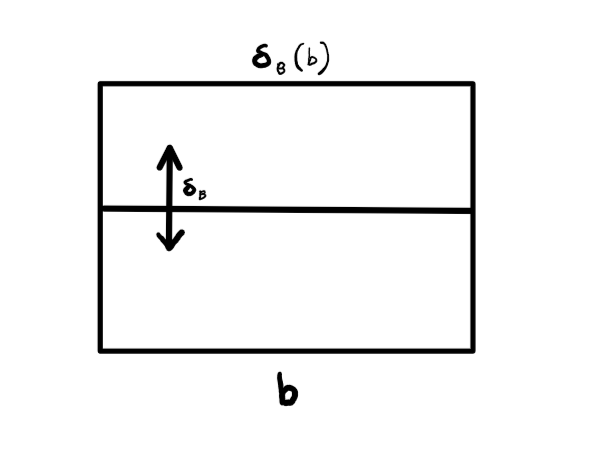
\includegraphics[width=0.5\linewidth]{sections/lorna/Band.png}
    \caption{A band}
    \label{band}
\end{figure}

\begin{definition}
    Let $\Gamma$ be a metric graph and $\mathcal{B}$ be a finite collection of bands. For each base $b$ of a band $B\in \mathcal{B}$ let $f_b:b\rightarrow\Gamma$ be an isometry such that $b$ is mapped into an edge of $\Gamma$ ($f_b(b)$ may be the whole edge or just part of it). A \emph{union of bands} is a space \[Y=\Gamma\cup\underset{B\in\mathcal{B}}{\bigsqcup}B/b \sim f_b(b).\] A \emph{leaf} of $Y$ is an equivalence class of points in $Y$ where two points are equivalent if they are in the same vertical fibre of a band in $Y$. See Figure \ref{unionofbands}.
\end{definition}
\begin{figure}[h]
    \centering
    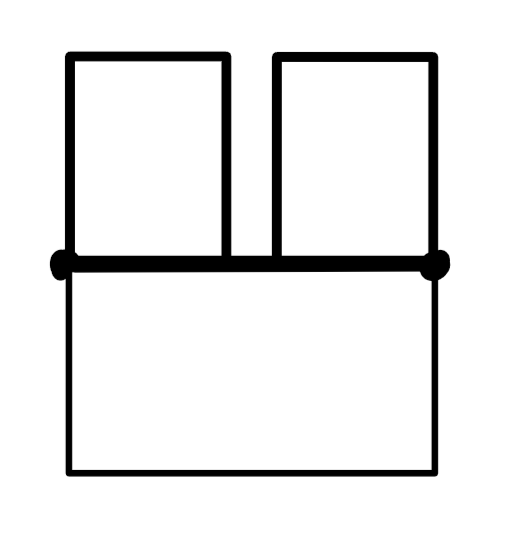
\includegraphics[width=0.4\linewidth]{sections/lorna/Union of Bands.png}
    \caption{A union of bands. The underlying graph is shown in bold.}
    \label{unionofbands}
\end{figure}

In some sources, the decomposition of a band complex $Y$ into leaves is called a \textit{foliation}.

\begin{definition}
    A measure $\mu$ on a metric space $X$ is \emph{transverse} to a measurable subset $S\subset X$ if 
    \begin{itemize}
        \item There is some compact subset $K$ of $V$ such that $0<\mu(K)<\infty$, and
        \item $\mu(v+S)=0$ for all $v\in V$.
    \end{itemize}
\end{definition}

\begin{lemma}\label{Ymeasure}
    Let $Y$ be a union of bands. Then there is a measure on $Y$ which is transverse to the leaves of the bands in $Y$.
\end{lemma}
\begin{proof}
     Let $\alpha$ be a path in a band $B$ with base $b$. $\alpha$ is \textit{transversal} if the projection of the image of $\alpha$ onto $b$ is injective, and its image is \textit{vertical} if it is contained in a single leaf. Define a measure $\mu$ on $Y$ as follows: If $\alpha$ is transverse, set $\mu(\alpha)=\ell(\alpha)$, and if the image of $\alpha$ is vertical, set $\mu(\alpha)=0$. Now for any path $\alpha:I\rightarrow V$, divide $I$ into intervals $I_j$ such that $\alpha\vert_{I_j}$ is either transversal or has vertical image. Then set \[\mu(\alpha)=\underset{j}\sum\alpha\vert_{I_j}.\] Then $\mu$ is clearly positive on any transversal path, but 0 on each of the leaves, as required.
\end{proof}


\begin{definition}
    Let $Y$ be a union of bands over a metric graph $\Gamma$. A \emph{band complex} $X$ is a relative CW 2-complex based on $Y$ such that:
    \begin{itemize}
        \item The 1-cells of $X$ are contained in $\Gamma$,
        \item The 2-cells meet $\Gamma$ at discrete sets, and
        \item The 2-cells intersect the bands along vertical sets.
    \end{itemize}
    See Figure \ref{bandcplx}.
\end{definition}

\begin{figure}[h]
    \centering
    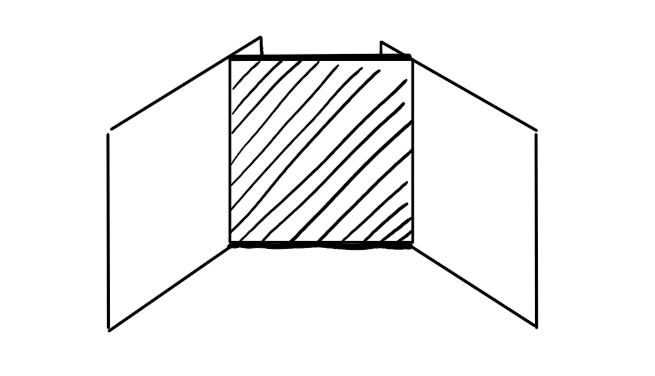
\includegraphics[width=0.6\linewidth]{sections/lorna/Band Complex.png}
    \caption{A band complex. There are two bands (unshaded), two 1-cells (in bold), and one 2-cell (shaded).}
    \label{bandcplx}
\end{figure}

\begin{lemma}
    Let $X$ be a band complex. Then $X$ admits a transverse measure. 
\end{lemma}
\begin{proof}
    As in the proof of \ref{Ymeasure}, a path $\alpha:I\rightarrow X$ can be divided up into subpaths $I_j$. Each of these subpaths is either transversal or vertical as before, or its image is contained in the closure of $X\backslash Y$. In the last case, define $\mu(\alpha\vert_{I_j})=0$.
\end{proof}

Let $X$ be a band complex. The leaves of $X$ are again defined as equivalence classes of points, here $x$ and $y$ are equivalent if there is a path of measure 0 from $x$ to $y$. 

Two points $\tilde{x}$ and $\tilde{y}$ in the universal cover $\tilde{X}$ of $X$ are in the same leaf if there is a path from $\tilde{x}$ to $\tilde{y}$ which projects to a path of measure 0 in $X$. 

\begin{definition}
    Let $G$ be a finitely generated group acting on an $\mathbb{R}$-tree $T$. A \emph{resolution} of the action is a band complex $X$ with $G$ as its fundamental group, and a $G$-equivariant map \[f:\tilde{X}\rightarrow T\] such that 
    \begin{itemize}
        \item The image of a leaf of $\tilde{X}$ is a point, and
        \item each base can be broken into finitely many subintervals whose lifts $f$ embed isometrically into $T$.
    \end{itemize}
\end{definition}


\begin{theorem}
    Let $G$ be a finitely presented group acting on an $\mathbb{R}$-tree $T$. Then the action has a resolution.
\end{theorem}
See \cite{Wilton} for the proof of this. The idea is that since $G$ is finitely presented there is a simplicial 2-complex $X$ with fundamental group $G$. A band complex structure on $X$ satisfying the required conditions can then be constructed.

In unpublished work in around 1991, Rips introduced an algorithm for determining certain properties of a group $G$ on an $\mathbb{R}$-tree from a resolving band complex for the action. This is now known as the \textit{Rips Machine}. We will give an outline of the process, followed by an idea of the consequences. More detailed descriptions are given in \cite{Wilton} and \cite{Bestvina_trees}.

Firstly, there are six moves $M0-M5$ on a band complex $X$ (based on a union of bands $Y$) which transform it into a band complex which resolves the same action but is minimal in some sense. These are:
\begin{itemize}
    \item $(M0)$: Attach a 2-cell to $X$ along a loop which is null-homotopic in $X$ but vertical in $Y\cup X^{(1)}$,
    \item $(M1)$: Add an annulus $B$ to $X$ along a subarc of the base graph $\Gamma$, then attach a 2-cell along a leaf of $B$,
    \item $(M2)$: Split a band $B$ down a leaf, and `fill in' the gap with a 2-cell,
    \item $(M3)$: Split a point not in any bases into a union of 1-cells,
    \item $(M4)$: `Slide' a band $B$ along another band $C$ such that its base moves from one base of $C$ to the other,
    \item $(M5)$: `Collapse' a band from a certain kind of subarc of a base.
\end{itemize}

The Rips Machine starts by repeatedly applying these moves to transform a connected component of a band complex $X$ into a minimal form. It then applies an infinite sequence of two `processes', and depending on which sequence is applied, information about the group can be determined. The following is Theorem 5.1 in \cite{Bestvina_trees}:

\begin{theorem}
    \textbf{Rips' theorem:} Let $G$ be a finitely generated torsion free group acting by isometries on an $\mathbb{R}$-tree $T$. Then applying the Rips Machine to a resolving band complex $X$ for the action, a band complex $X'$ is obtained which can be split into disjoint components $X'_i$ such that each $X'_i$ is of one of the following types:
    \begin{itemize}
        \item \emph{Simplicial} - Every leaf of the underlying union of bands of $X'_i$ is compact,
        \item \emph{Surface type} - $X'_i$ is a compact surface with negative Euler characteristic,
        \item \emph{Toral type} - $X'_i$ is the 2-skeleton of the torus,
        \item \emph{Thin type} - $X'_i$ is not of one of the above types.
    \end{itemize}
\end{theorem}

This theorem allows us to classify finitely presented groups which act `nicely' on $\mathbb{R}$-trees.
\begin{theorem}\label{rtreesclassification}
    Let $G$ be a finitely generated torsion-free group acting non-trivially by isometries on an $\mathbb{R}$-tree $T$. Suppose also that all arc stabilizers are trivial. Then one of the following holds:
    \begin{enumerate}
        \item $G$ is the fundamental group of a 2-complex $X$ which contains a compact surface $S$ of negative Euler characterisic,
        \item $G$ is a free abelian group,
        \item $G$ splits as a non-trivial free product. Each free factor also acts on $T$, and either stabilises a point (so in particular contains only elliptic elements), or this theorem may be applied again to the factor.
    \end{enumerate}
\end{theorem}
\begin{proof} (Sketch)
    Start by applying the Rips Machine to a resolving band complex for the action to get a band complex $X'$. 

    Clearly if $X'$ has a component of surface type, possibility (1) holds.

    If $X'$ has a component $X'_i$ of toral type, either \[G=\pi_1(X'_i)=\pi_1(\mathbb{T}_2)=\mathbb{Z}\times\mathbb{Z}\] which is a free abelian group, or a free product decomposition can be obtained using the boundary of $X'_i$. So either possibility (2) or (3) holds. 

    If $X'$ has a component $X'_i$ of thin type, it can be shown that the Rips Machine subdivides some band repeatedly into thinner and thinner bands. Some of these bands will eventually be disjoint from any of the 2-cells of $X'$. These bands are called \textit{naked bands} and induce free product decompositions of $\pi_1(X')$ \textcolor{red}{could give more detail here?}\todo[color=green!40]{I don't think it's needed!}. Hence possibility (3) holds.

    Finally, if $X'$ has a simplicial component $X'_i$, an $\mathbb{R}$-tree \textit{dual} to $X'_i$ can be constructed, on which $G$ acts. Bass-Serre theory can then be used to show that $G$ splits as a non-trivial free product.
\end{proof}

The next theorem tells us what happens in the slightly more general case of groups acting freely on $\mathbb{R}$-trees. \todo[color=green!40]{I would either move this to directly before the theorem. The reader could expect a theorem immediately ahead and be confused to see a definition!}
\begin{definition}
    A group $G$ is a \emph{closed surface group} if it is the fundamental group of a closed surface. For example the groups in case (1) of the previous theorem are closed surface groups.
\end{definition}
\begin{definition}
    A group $G$ is \emph{freely indecomposable} if it is nontrivial and cannot be expressed as a free product of nontrivial groups.
\end{definition}

\begin{theorem}
    Let $G$ be a finitely presented group acting freely by isometries on an $\mathbb{R}$-tree $T$. Then $G$ is the free product of free abelian groups and closed surface groups.
\end{theorem}
\begin{proof}
    $G$ can be written as the free product of a free group and a number of freely indecomposable factors. It can be shown that each of these factors satisfies the conditions of Theorem \ref{rtreesclassification}, and by assumption neither possibility (2) nor (3) holds, so each freely indecomposable factor must be a closed surface group. 
\end{proof}

Finally, we see the case of stable actions. The proof of the following theorem can be found in \cite{Bestvina2}.

\begin{theorem}\label{stable}
    Let $G$ be a finitely presented group with a stable action on an $\mathbb{R}$-tree $T$. Then either
    \begin{itemize}
        \item $G$ splits over an $E$-by-cyclic extension where $E$ fixes some arc of $T$, or
        \item $T$ is a line, and $G$ splits over an extension of the kernel of the action by a free abelian group.
    \end{itemize}
\end{theorem}

\subsection{Applications of $\mathbb{R}$-Trees}
Now that we have a good understanding of groups which act (freely) on $\mathbb{R}$-trees, we can use this to understand any group which can be shown to act in this way. In this section we will discuss some of these applications, starting with some to hyperbolic groups.

\begin{theorem}
    Let $G$ be a hyperbolic group such that Out$(G)$ is infinite. Then $G$ splits over a virtually cyclic subgroup.
\end{theorem}

\begin{proof} (sketch)
    Since Out$(G)$ is infinite, we can find an infinite sequence of pairwise non-conjugate automorphisms $f_i$. Define an action $\rho_i$ of $G$ on its Cayley graph by $\rho_i(g)=f_i(g)$. \todo[color=green!40]{Perhaps you could add ``As the \(f_i\) are automorphisms,\dots,'' or something which justifies why it is easily seen.}It is easily seen that this is an action by isometries. Theorem \ref{limittrees} can then be used to show that there is a limit $\mathbb{R}$-tree on which $G$ acts by isometries. It can then be shown that this action is stable, and the theorem follows by Theorem \ref{stable}. See \cite{BridsonSwarup} for a more detailed proof.
\end{proof}

$\mathbb{R}$-trees are also instrumental in the study of Culler and Vogtmann's \textit{Outer Space}. We will give a brief overview of this subject. For more detail see section 2 of \cite{Shalen}.

\begin{definition}
    The action of a group $G$ on an $\mathbb{R}$-tree is \emph{polyhedral} if it is topologically equivalent to a simplicial action.
\end{definition}
\begin{definition}
    For a group acting by isometries on an $\mathbb{R}$-tree, the function $l:G\rightarrow\mathbb{R}$ given by $l(g)=\lVert g\rVert$ is called the \emph{length function} associated to the action.
\end{definition}

Let $\mathcal{L}(G)$ denote the set of all length functions for non-trivial actions of $G$ on $\mathbb{R}$-trees. Quotienting out by the obvious action of $\mathbb{R}$ gives the space $\mathcal{PL}(G)$ of \textit{projectivised length functions}. Let $F_n$ be the free group on $n$ generators, and $Y_n\subseteq \mathcal{PL}(F_n)$ the set of projectivised length functions defined by polyhedral actions. The space $Y_n$ is known as \textit{outer space}, as it admits a `nice' action of Out$(F_n)$. 

There is a theorem in Bass-Serre theory which states that a group is free if and only if it acts freely on a simplicial tree. The theory of outer space can be used to study free actions of free groups on $\mathbb{R}$-trees. In the $n=2$ case, it has been shown that the only free actions of $F_2$ on $\mathbb{R}$-trees are polyhedral, i.e. their length functions are in $Y_2$. For every $n\geq 3$ however, one can show that the set $\bar{Y}_n\backslash Y_n$ (where $\bar{Y}_n$ denotes the closure of $Y_n$ in $\mathcal{PL}(F_n)$) contains free actions. Therefore there are free actions of $F_n$ on $\mathbb{R}$-trees which are not polyhedral, sometimes referred to as \textit{exotic} actions. This demonstrates another key difference between simplicial trees and the slightly more general class of $\mathbb{R}$-trees.


We finish with another application to hyperbolic groups.
\begin{definition}
    A topological space $X$ is \emph{locally connected} at $x\in X$ if every open neighbourhood of $x$ contains a connected open neighbourhood of $x$. $X$ is locally connected if it is locally connected at all of its points.
\end{definition}
Note first that neither connected nor locally connected implies the other: the union of two disjoint intervals in $\mathbb{R}$ is locally connected but not connected, whereas the graph of $\sin(\frac{1}{x})$ is connected but not locally connected.

\begin{theorem}
    Let $G$ be a hyperbolic group. Then if $G$ has one end, its Gromov boundary $\partial G$ is connected and locally connected.
\end{theorem}

The proof of this can be found in \textcolor{red}{???}. See the next section for more about ends of groups.\todo[color=green!40]{I think in the new order, your section will be the final one so just remember to take this out! Will go over the maths more carefully next week and leave some small comments hopefully on Monday.}




